\documentclass{article}

\usepackage{graphicx}
\usepackage[margin=1in]{geometry}

\title{A Calculus Formula and Plot}
\author{}
\date{}

\begin{document}

\maketitle

Below is a formula \(x^2\).

The displayed formula is

\[
x^2
\]

Figure~\ref{fig:xsquared} shows the graph of \(y=x^2\) for
\(-2 \leq x \leq 2\).

\begin{figure}[htbp]
 \centering
 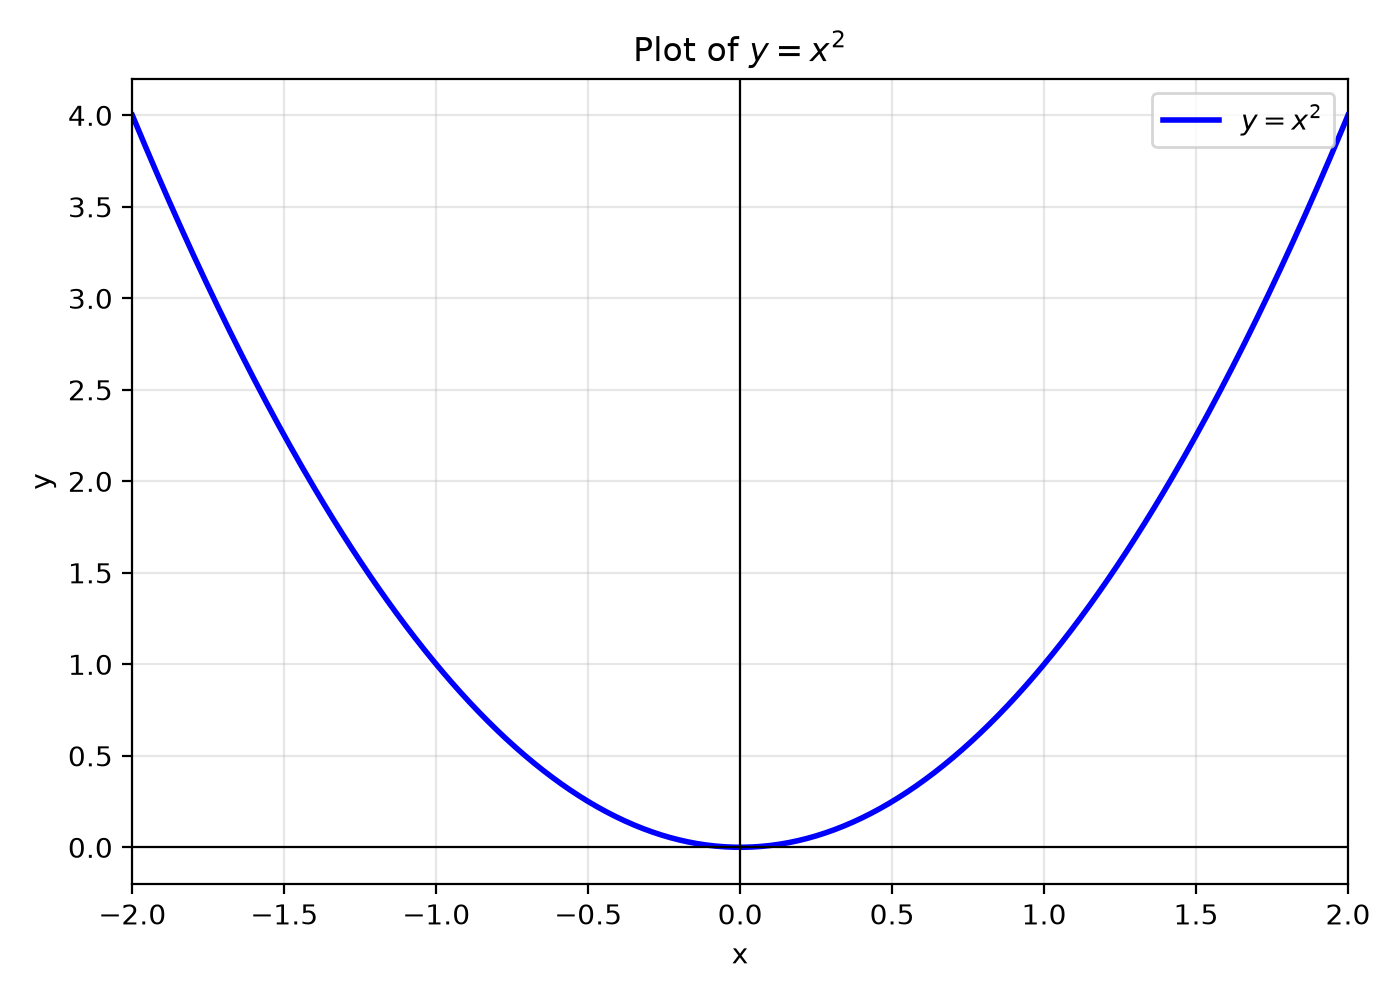
\includegraphics[width=0.8\textwidth]{f1.png}
 \caption{The graph of \(y=x^2\) on the interval \([-2,2]\).}
 \label{fig:xsquared}
\end{figure}

\end{document}
